\documentclass{article}
\usepackage{graphicx}
\usepackage{url}
\begin{document}
\begin{center}
\title{Prediction Of Arrival Of Nodes In\\\ Scale Free Networks}
\maketitle
\end{center}
\begin{abstract}
$\cal R$ecent observations in the development of the scale free networks posed several questions. Few characteristics of these graphs are thought to serve specific purposes that can have significant impact on mankind. One such unsolved mystery is determining the chronology in scale free network. The motivation is, can we predict the evolution of network? Is there an organized way of determining the order of arrival of vertices in a Scale Free Network? Here we propose a model which analyses the network’s characteristics, the properties of nodes to answers these questions, demonstrating the idea of the growth of a network. 
\end{abstract}
\section{Introduction}
\hspace{.17in} $\cal L$ately we have been able to recognize networks in day to day life. It ranges widely from simple ecosystems to complex brain networks, from social networks to the World Wide Web, from air networks to citation networks and the list goes on. The questions that pop up are, are all these real world networks randomly generated? Do they follow the \emph{Poisson distribution}\cite{pois}? If these questions were posed a decade ago, the answer would have been probably yes. 
%\emph{Random graph} follows Poisson distribution that is there are many vertices having approximately same number of links which is average degree of the graph and very few vertices deviate from the average (Deviation is less). 
Due to avalanche of research on this real world graphs, it has been proved that the degree distribution of the vertices doesn't obey Gaussian distribution\cite{bara1}. In fact they follow a common paradigm which is nothing but the power law distribution of degree. The term Scale-Free was coined to describe this pattern.\cite{bara1} 

Justifications for this behavior were growth and preferential attachment. Real world networks are rapidly expanding and are dynamic in nature. For example, the web which was just one page when it started has shot up to billions now. Another prominent reason is the preference factor in the real world networks. An incoming node prefers a popular node (A node with high degree) over the other. 'Rich gets Richer' is the key that unravels the mystery of preferential attachment that the network follows. Growth combined with the preferential attachment explains the scale free nature.
        %$\cal A$ scale free network follows \emph{Power law distribution}. 

Scale free networks $G=(V,C)$ follow a common pattern which is random network formation linked with preferential attachment exhibits the power law distribution of degree.
\begin{equation}
\fbox{$\bf P(k) \approx ck ^{-\gamma} | k>C$} 
\end{equation}
where, \\
\textbf{k} is \emph{degree},\\ 
\hspace{.18in}\textbf{c}  is a \emph{normalization constant} and \\
\textbf{$\gamma$} is a \emph{parameter} whose value is typically in the range 
\begin{equation}
\fbox{$\bf 2 <\gamma <3$}
\end{equation}
\begin{figure}[htp]
\centering
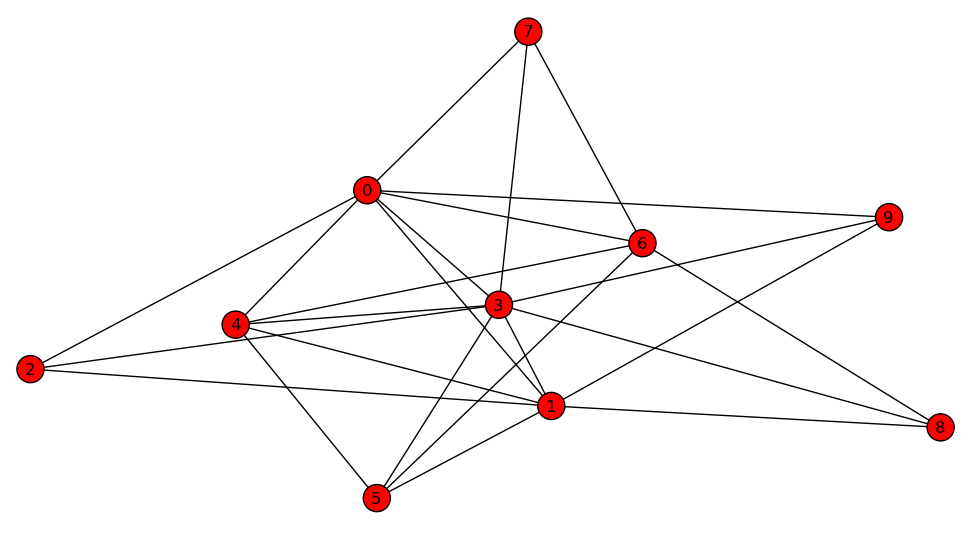
\includegraphics[scale=0.30]{Figures/LabelledNetwork.png}
\caption{A scale free network Of 10 nodes, 3 connections}
\label{}
\end{figure}

Understanding the characteristics of scale free networks in depth helps us realize the fact that the cell network, friendship network, genetic network are no way different from the scale free category. In fact, exploring these networks can actually play a vital role in understanding the interactions and curing of several faulty nodes in a complex protein network that causes cancer. A small contribution in this direction that can open up several more questions is predicting the order in which nodes arrive in the network which we call the \bf \emph{Prediction Problem}\rm .

Look at the information that can be extracted from the given $G = (V,C)$ undirected unweighted scale free  network whose prediction is to be determined. $|V|$ number of nodes and $D_i$ degree of vertex where $i \in V$ can be inferred by visualizing the graph. The fact that the degree distribution in scale free networks follows powerlaw distribution compels us to conclude that the vertex with higher degree has arrived before the one with the lower degree. But there exists many vertices with the same degree. Hence, there is no perceptible way of
prediction among vertices having the same degree.

Hence we consider a hypothetical container called \bf \emph{Bin} \rm to place all such nodes whose arrival among themselves is not known but prediction across several such Bins can be determined. Let $ \delta $ \emph{\textbf{the number of bins}}, $\xi $ \textbf{\emph{number of nodes in each bin on an average}} $ i.e $ $\xi = \frac {|V|}{\delta}$ and  $\eta$ be \emph{\textbf{the accuracy}} the associated with the prediction. Binning based on degree results in low $\delta$,$\eta$ value and high value of $\xi$   
\\\
\begin{figure}[htp]
\centering
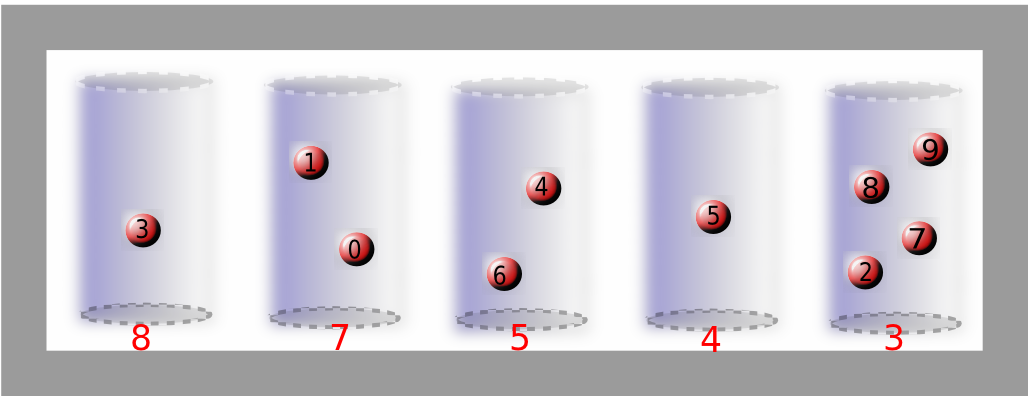
\includegraphics[scale=0.35]{Figures/bins.png}
\caption{Binning nodes based on degree from figure 1. Where node '3' is of degree(8), Nodes '1' and '0' is of degree(7) , Nodes '4' and '6' is of degree(5), Node '5' is of Degree(5) , Nodes '9','8','7','2' is of degree(3).}
\label{}
\end{figure}
\begin{figure}[htp]
\centering
\includegraphics[scale=0.22]{Figures/1000_3_powerlaw.png}
\caption{Demonstrates the number of nodes in each Bin (follows Power Law Of Distribution) of $G = (1000, 3)$.The first peak at $3^{rd}$ unit indicates at the first bin has 400 nodes, second peak at $4^{th}$ unit indicates that second bin has 200 nodes, and so on.}
\label{}
\end{figure}

\emph{$\cal T$he \emph{\textbf{aim}} of this problem is to maximize the number of bins ($\delta$) and minimize the elements inside the bins($\xi$). with a accurate prediction($\eta$).Which is nothing but optimum solution
}

\newpage 

$\cal I$n this paper,  initially we intend to simulate the given network to the maximum possible extent. Since it is intricate to corral such a accurate replication we generate as many sample graphs possible. Each sharing few characteristics of the \emph{Main model}. Since the ordering in the sample set is known in prior while generating them, we map the nodes of the sample set with corresponding nodes of the main model based on the certain properties of the node. Prediction lists i.e. the complete ordering of the vertices are obtained from each of the sample graph generated  by mapping which are used for further processing to fine-tune the accuracy. The method demonstrated in this paper provides appreciable number of bins for a given scale free network.

\section{Preliminaries}
\subsection{Graph}
\hspace{.18in} $\cal A$ graph is an abstract representation of a set of objects where some pairs of the objects are connected by links. The interconnected objects are represented by mathematical abstractions called \emph{vertices}, and the \emph{links} that connect some pairs of vertices are called \emph{edges}.
\subsection{Scale Free Networks}
\hspace{.18in} $\cal A$ class of real world networks whose degree distribution follows power law\cite{bara1}.
\subsubsection{Nodes \& Connections In A Scale Free Network}
\hspace{.18in}$\cal N$odes are number of vertices in the network, Connections are the number of links a node make when it enters the network.
\subsubsection{Generative Procedure For Scale Free Network $G=(V,C)$}
\begin{enumerate}
\item \textbf{Inputs} : $\cal W$here $C$ be the number of links to add to each new node and $|V|$ be the network size i.e. the number of nodes.
\item \textbf{Initialize} : $\cal D$esignate nodes by enumerating them as        $0,1,2, . . . , (n-1)$, given the number of nodes $ n > C $. Initially construct a complete network with $C$ Nodes. The degree sequence of this complete network is $\{(C-1),(C-1),(C-1),...\}$.set $ nNodes=C$
\item While $nNodes<=|V|$ :
\begin{enumerate}
\item \textbf{New node}: $\cal G$enerate a new node v.
\item \textbf{New links} : $\cal S $et $nlinks =  minimum (C, |V|)$. Cannot add more links than existing nodes.
\item Repeat $nlinks$ times:
\begin{enumerate}
\item \bf Preferential attachment \rm :$\cal S$elect an existing node u by sampling from the cumulative degree sequence distribution function $CDF(i)$ defined by :
\begin{equation}
CDF(i) =\sum^{i}_{j}\frac{degree(Nj)}{2*total\_edges}\ \ where\ N_j \in V
\end{equation} 
\item \cal Let r be a uniform random number from [0,1). Then u is a random variable sampled from $CDF(i)$ as follows:
\begin{equation}
CDF(u-1)  <= r <= CDF(u)
\end{equation}
\begin{equation}
where\ u =r*nNodes
\end{equation}

\item \cal Connect $v~u$, Avoid duplicate links.In-case if duplicate link occurs remove the link, reduce $nlinks$ by one and redo the steps from 3.c
\end{enumerate}
\end{enumerate}
\end{enumerate}

\begin{figure}[htp]
\centering
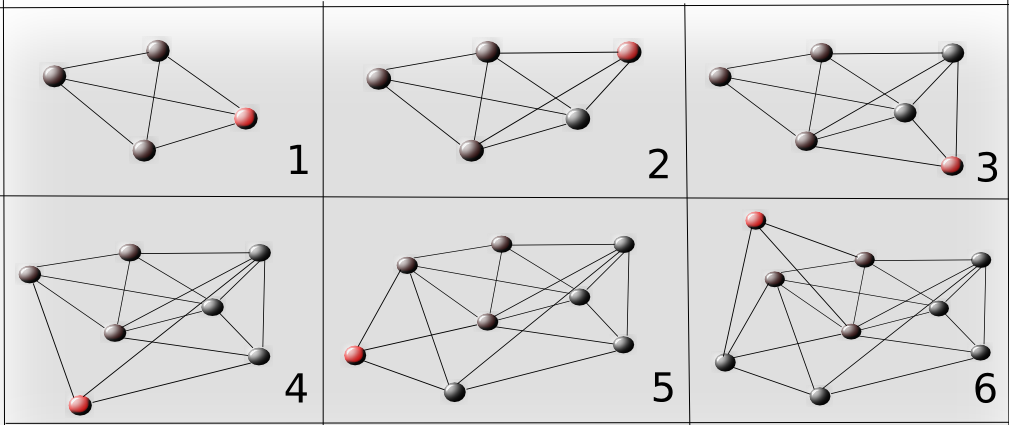
\includegraphics[scale=0.35]{Figures/ScaleFreeNetwork.png}
\caption{Formation of Scale Free Network $G=(9,3)$.Red node is a new node entering the network and attaching to the existing nodes(Black nodes)}
\label{}
\end{figure}

\subsection{Hubs In A Scale Free Network}
\hspace{.18in}$\cal T$he variety of complex systems share a important property. Some nodes have a tremendous number of connections to other nodes. These popular nodes are called \emph{Hubs}. In Figure 1,node '3' acts as Hub. 
\subsection{Main Model}
\hspace{.18in}$G_m = (V_m,C_m)$ is the subject of our experiment(Main Model). Where $V_m$ is the number of nodes in this network and $C_m$ as Connections. Whose order of arrival of nodes has to be found out.
\subsection{Directed Acyclic Graph}
\hspace{.18in}$\cal A$ directed acyclic graph, is a directed graph. That is, it is formed by a collection of vertices and directed edges, each edge connecting one vertex to another, such that there is no way to start at some vertex $v$ and follow a sequence of edges that eventually loops back to $v$ again.
\subsection{In-degree} 
\hspace{.18in} $\cal T$he number of head endpoints adjacent to a node in a directed graph is called the in-degree of the node.

$Indegree_v = |S|\ such\ that\ S = \{(u,v)|u,v \in E(G)\}$

\subsection{Out-degree}
\hspace{.18in} $\cal T$he number of tail endpoints in a directed graph is out-degree.

$Outdegree_v = |S|\ such\ that\ S = \{(v,u)|v,u \in E(G)\}$

\subsection{Prediction List}
\hspace{.18in}$\cal A$ list that contains all the nodes in the order of their arrival   
\subsection{Rank of a Node}
\hspace{.18in}$\cal I$n the chronology of arrival of nodes in a network. The position of the node is the ranking associated with it.  
\subsection{Centrality Measures}
\hspace{.18in} $\cal A$ vertex centrality is a real-valued function assigning to each vertex in a network some value. Higher the value, more central or important the vertex is for the  network. This function when applied to a graph, it gives out the centrality values for each vertex.
\subsubsection{Degree Centrality}
\hspace{.18in} $\cal T$he degree centrality of a node in a network is based on the number of nodes it has as its immediate neighbours(Degree).Mathematically for a graph $G = (V,C)$,where V is the vertex set of graph,C connections is given as:
\begin{equation}
C_{degree}(v) = \frac{deg(v)}{|V|-1}
\hspace{.4in} v \in V
\end{equation} 
\subsubsection{Betweenness Centrality}
\hspace{.18in} $\cal L$et \rm$\delta(v)$ denote the fraction of shortest paths between $s$ and $t$ that contain the vertex $v$:
\begin{equation}
\delta_{st} = \frac{\sigma_{st}(v)}{\sigma_{st}} 
\end{equation}
where $\sigma_{st}$ denotes number of all shortest path from vertex $s$ to $t$ and $\sigma_{st}(v)$ denotes the number of shortest path from $s$ to $t$ passing through $v$. Then the Betweenness centrality $BC(v)$ of a vertex $v$ is given by 
\begin{equation}
C_{betweenness}(v) = \sum_{s\neq v \neq t \in G} \delta_{st}(v)
\end{equation}
\subsubsection{Eigenvector Centrality}
\hspace{.18in} $\cal T$he index in Eigen-Vector centrality characterizes individuals in connected networks according to their level of popularity. A given individual is said to be popular if he is connected to many individuals or few individuals with a very high popularity. It assigns relative scores to all nodes in the network based on the principle that connections to high-scoring nodes contribute more to the score of the node in question than equal connections to low-scoring nodes. Mathematically, this can be written as follows:

Let $ A_{i,j}$ be the adjacency matrix of the network. Where $A_{i,j}=1$ if there is a edge between $i^{th}$ node and $j^{th}$ node else $A_{i,j}$ is set to $0$.

Let $x_i$ denote the score of the $i^{th}$ node.

For the $i^{th}$ node, let the centrality score be proportional to the sum of the scores of all nodes which are connected to it. Hence
\begin{equation}
x_{i} = \frac{1}{\lambda} \sum_{j \in M(i)} x_i = \frac{1}{\lambda} \sum_{j=1}^{N} A_{i,j} x_j
\end{equation}

Where $M(i)$ is the set of nodes connected to $i^{th}$ node, Where $N = |V|$ is the number of nodes and $\lambda$ is a constant. In the vector notation this can be written as 
\begin{equation}
x = \frac{1}{\lambda} A x
\end{equation} 
In general, there will be many different eigenvalues $\lambda$ for which an eigenvector solution exists. However, the additional requirement that all the entries in the eigenvector be positive implies (by the Perron–Frobenius theorem)[cite] that only the greatest eigenvalue results in the desired centrality measure. The $i^{th}$ component of the related eigenvector then gives the centrality score of the $i^{th}$ node in the network. Power iteration is one of many eigenvalue algorithms that may be used to find this dominant eigenvector.
\subsection{Plain Centrality Ranking}
\hspace{.18in}$\cal W$hen any centrality measure $\chi$ is applied to a graph. It gives a value to each and ever node based on how important it is in the network. Deriving a prediction list from the centrality values in there decreasing order. The rank assigned to each node by this method is called as Plain Centrality Ranking.
\subsection{Differential Core Ranking}
\hspace{.18in}$\cal D$ifferential Core Ranking is used to concretize the prediction of arrival of vertices. It adopts the method of assigning values to the nodes by adding the continuous differences in their centrality values on the removal of certain nodes in the graphs successively until there are no nodes left in the graph. Consider a graph $G(V,C)$. Let $\chi$ be any centrality (from section 2.8) that is applied on the graph G. Let $G_0$ be the initial graph. Let $G_1$ be the graph obtained from $G_0$ after removal of certain nodes, $G_2$ be the graph obtained from $G_1$ after removal of certain nodes and so on. In general, let $G_{i+1}$ be the graph obtained after removal of certain nodes from $G_i$.

At each step in the algorithm, remove the nodes with the least differential centrality value from $G_i$ to get $G_{i+1}$. Apply the centrality measure $\chi$ to $G_{i+1}$. We get centralities recomputed for the nodes in $G_{i+1}$.The idea is that the least affected node is the one that has come the earliest, and lasts till the end. Hence, there is a need to compute the change in centrality for each node in $G_{i+1}$.the nodes removed at each step is given last chronological ranking.

\begin{figure}[htp]
\centering
\includegraphics[scale=0.22]{Figures/Diffrence_Plain_nodes_100_to_1000,5.png}
\caption{Comparing Differential Core Ranking(Blue line) vs. Plain Centrality Ranking(Green line) for varying number of nodes from 100 to 1000(x-axis), with constant connection as 5. y-axis denotes percentage accuracy in prediction}
\label{}
\end{figure}

\begin{figure}[htp]
\centering
\includegraphics[scale=0.22]{Figures/Diffrence_Plain_1000node,connection_5to12(2).png}
\caption{Comparing Differential Core Ranking(Blue line) vs. Plain Centrality Ranking(Green line) for graph of nodes 1000, with varying connection from 3 to 13 (x-axis). y-axis denotes percentage accuracy in prediction.}
\label{}
\end{figure}

\newpage

$\cal T$he plots clearly support the fact that prediction list obtained from the Differential Core Ranking, for any given centrality $\chi$, provides more accuracy compared to prediction list obtained from the Plain Centrality $\chi$.
%\newpage
\section{Trivial Methods}
\subsection{Delta Binning based on Degree}
\hspace{.17in}$\cal O$ne of the main highlight of a Scale free network is the formation of nodes with high degree, known as hubs. Such nodes though few in number, dominate the network to a great extent simply for the reason that removal of such nodes may cause the graph to get disconnected. By knowing how scale free networks are generated from the generative model above, with a high probability it can be said that the notable hubs would have come way before in comparison to the nodes with low degree. Based on Plain Degree Ranking we segregate the nodes into 2 different bins. Iteratively bin the nodes in 3 different bins. This procedure is done until we get $\delta$ number of bins which is such that each bin contains node having same degree. In each step of the procedure we apply a measure to find out the accuracy with which we can predict the order of the bins. In order to find out how accurate this is, we design a \textbf{\emph{Binning Quality Measure}}, which gives points on scale of 0 to 1 that would give the accuracy rate. It works as follows. 	
\\\

\textbf{ Score associated with a pair of bins }= $\beta$

\begin{equation}
\beta = \frac{number\ of\ hits\ comparing\ for\ every\ U\ in\ one\ bin\ with\ every\ V\ in\ another\ bin}{total\ number\ of\ comparisons}
\end{equation}

\emph{where U and V are any pair of vertices chosen from two different bins}.
\\\
 
\textbf{Hits} :  The number of times U  arrived before V.
\\\

\textbf{Misses} : The number of times V arrived before U.
\\\
\begin{equation}
\textbf{Binning\ Quality (Total\ Bin\ Score)} =\eta= \frac{\beta\ score\ for\ all\ ^\delta C_2\ bins}{^\delta C_2}
\end{equation}
\\\

\begin{figure}[htp]
\centering
\includegraphics[scale=0.24]{Figures/1000,3_delta_degree_binning2.png}
\caption{As the number of bins($\delta$) increases there is a decrease in bin measure($\eta$) for a barabasi graph $G(500,3)$. X-axis denotes the number of bins. Y-axis denotes the Binning Quality $\eta$}
\label{X axis : Number Of Bins , Y axis : Bin Measure}
\end{figure}

\rm From the plot(Figure 7) we can conclude that as the number of bins increases from 2 to $\delta$, the accuracy starts dipping. Further we can’t divide the bins beyond $\delta$ as prediction cannot be derived from the nodes with the same degree. Though the accuracy rate is fair enough applying the \emph{Bin Quality Measure}, we realize that in this method we get very few such bins and major portion of the prediction remains unachieved. This thrives us to discover other methods which could give us more promising results with more number of Bins.

\subsection{Delta Binning based on Centrality}
\hspace{.2in}$\cal T$he main drawback of the \it Delta Binning \rm was the small value of $\delta$ and $\eta$. We move on to yet another approach which could provide us with a large value of $\delta$. This approach is based on a intuitive conjecture that more important a node, the older it would have been present in that network. More important the node, earlier it has come with a high probability’ is the main motto behind this method.
There are various way of assigning importance to a node. This is where centralities come into picture. Various $\chi$ centralities are applied to the network and depending on the values given to each node we derive a \bf \emph{Prediction List}\rm.
The values given to nodes by the eigen ,betweenness centralities are mostly unique. This approach gives us a $\delta$ as high as the total number of nodes in the network. That’s nothing but one element in each bin. This is done over several trials and over many known centralities stretching from eigen to betweeness.

\begin{figure}[htp]
\centering
\includegraphics[scale=0.28]{Figures/1000,5comparing_degree_betwenness_eigen3.png}
\caption{Comparing Degree(green),Betweenness(blue),Eigenvector Centalities(red) as the $\delta$ increases. x-axis denotes the number of bins. y-axis denotes the accuracy $\eta$.}
\label{}
\end{figure}

Looking at the figure above we draw a conclusion that though this is giving us high value of delta the accuracy is still not up to the mark.

\section{Delta Binning based on DAG}
\hspace{.18in} $\cal O$ur method is a technique where in we apply iterative actions in order to obtain a Prediction List for the given Main Model. 

Its divided into 4 Main sections. 
Section 4.1 aims at creating sample space for the given scale free network.
Section 4.2 describes a mapping procedure to map each and every node of the main graph to nodes of each of the graphs in the sample space. The next section gives an approach to derive a prediction list after applying methodologies of the previous sections. The last section 4.4 provides an efficient way of Binning
\subsection{Generating the sample space}
\hspace{.17in}$\cal I$n this section, we intend to recreate the scene of generating Main Model. This is done by generating many graphs of the same kind by sharing few similarities of the Main Model. Taking a look at the Main Model, the simple information that can be extracted are the number of nodes and degree of each of the node. Further, deciding from the smallest degree in the Main graph, the connections ($C$) for sample graphs is chosen. Here we are generating $\alpha$ number of sample graphs which are supposed to be odd. The magnificence of these sample graphs is that we know the actual arrival sequence of each of these graphs which is a stepping stone towards our goal.
\subsection{Mapping}
\hspace{.17in} $\cal I$n this section we assign a rank to all the nodes of the main model with respect to each graph in the sample space. As all the graphs in the sample space are considered equivalent when it comes to sharing similarities with the main model, it is righteous to derive prediction list from all the graphs in the sample space. First let us look at the methodology in assigning the ranks. For simplicity we explain the procedure for a single graph, s-graph from the sample set space. The main step that aids this is establishing a rule of correspondence between nodes of the main model and each node in the s-graph.

The basis for this mapping is Differential Core Ranking. It is applied both to the main model and the sample graph and based on the values assigned; we derive 2 lists with nodes sorted in the descending order of their Differential core ranking values. From the 2 lists trivial one to one mapping is done, in the sense the node with highest differential ranking value in the main model is mapped to node with highest differential ranking value in the sample graph, also the node with second highest value in main graph with the 2nd highest value node in sample graph and so on. The rank of the vertex associated with a node in the sample graph is assigned to its corresponding node in main model as the outcome of mapping. With all the ranks assigned we get the prediction list.

\begin{figure}[htp]
\centering
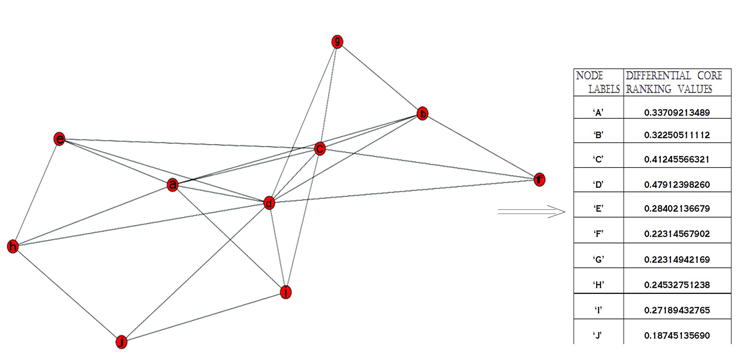
\includegraphics[scale=0.13]{Figures/Mapping_Graph1.jpg}
\caption{Applying Differential core centrality(with $\chi$ as betweenness centrality) to Main Graph assigns each node with a unique value.}
\label{}
\end{figure}

\begin{figure}[htp]
\centering
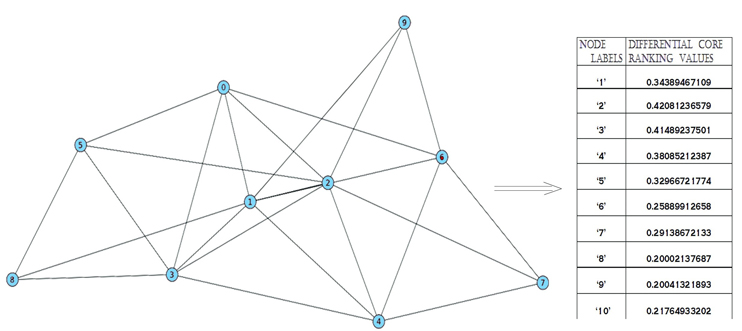
\includegraphics[scale=0.14]{Figures/Mapping_Graph2.jpg}
\caption{Applying Differential core centrality (with $\chi$ as betweenness centrality) to Sample Graph assigns each node with a unique value.}
\label{}
\end{figure}

\begin{figure}[htp]
\centering
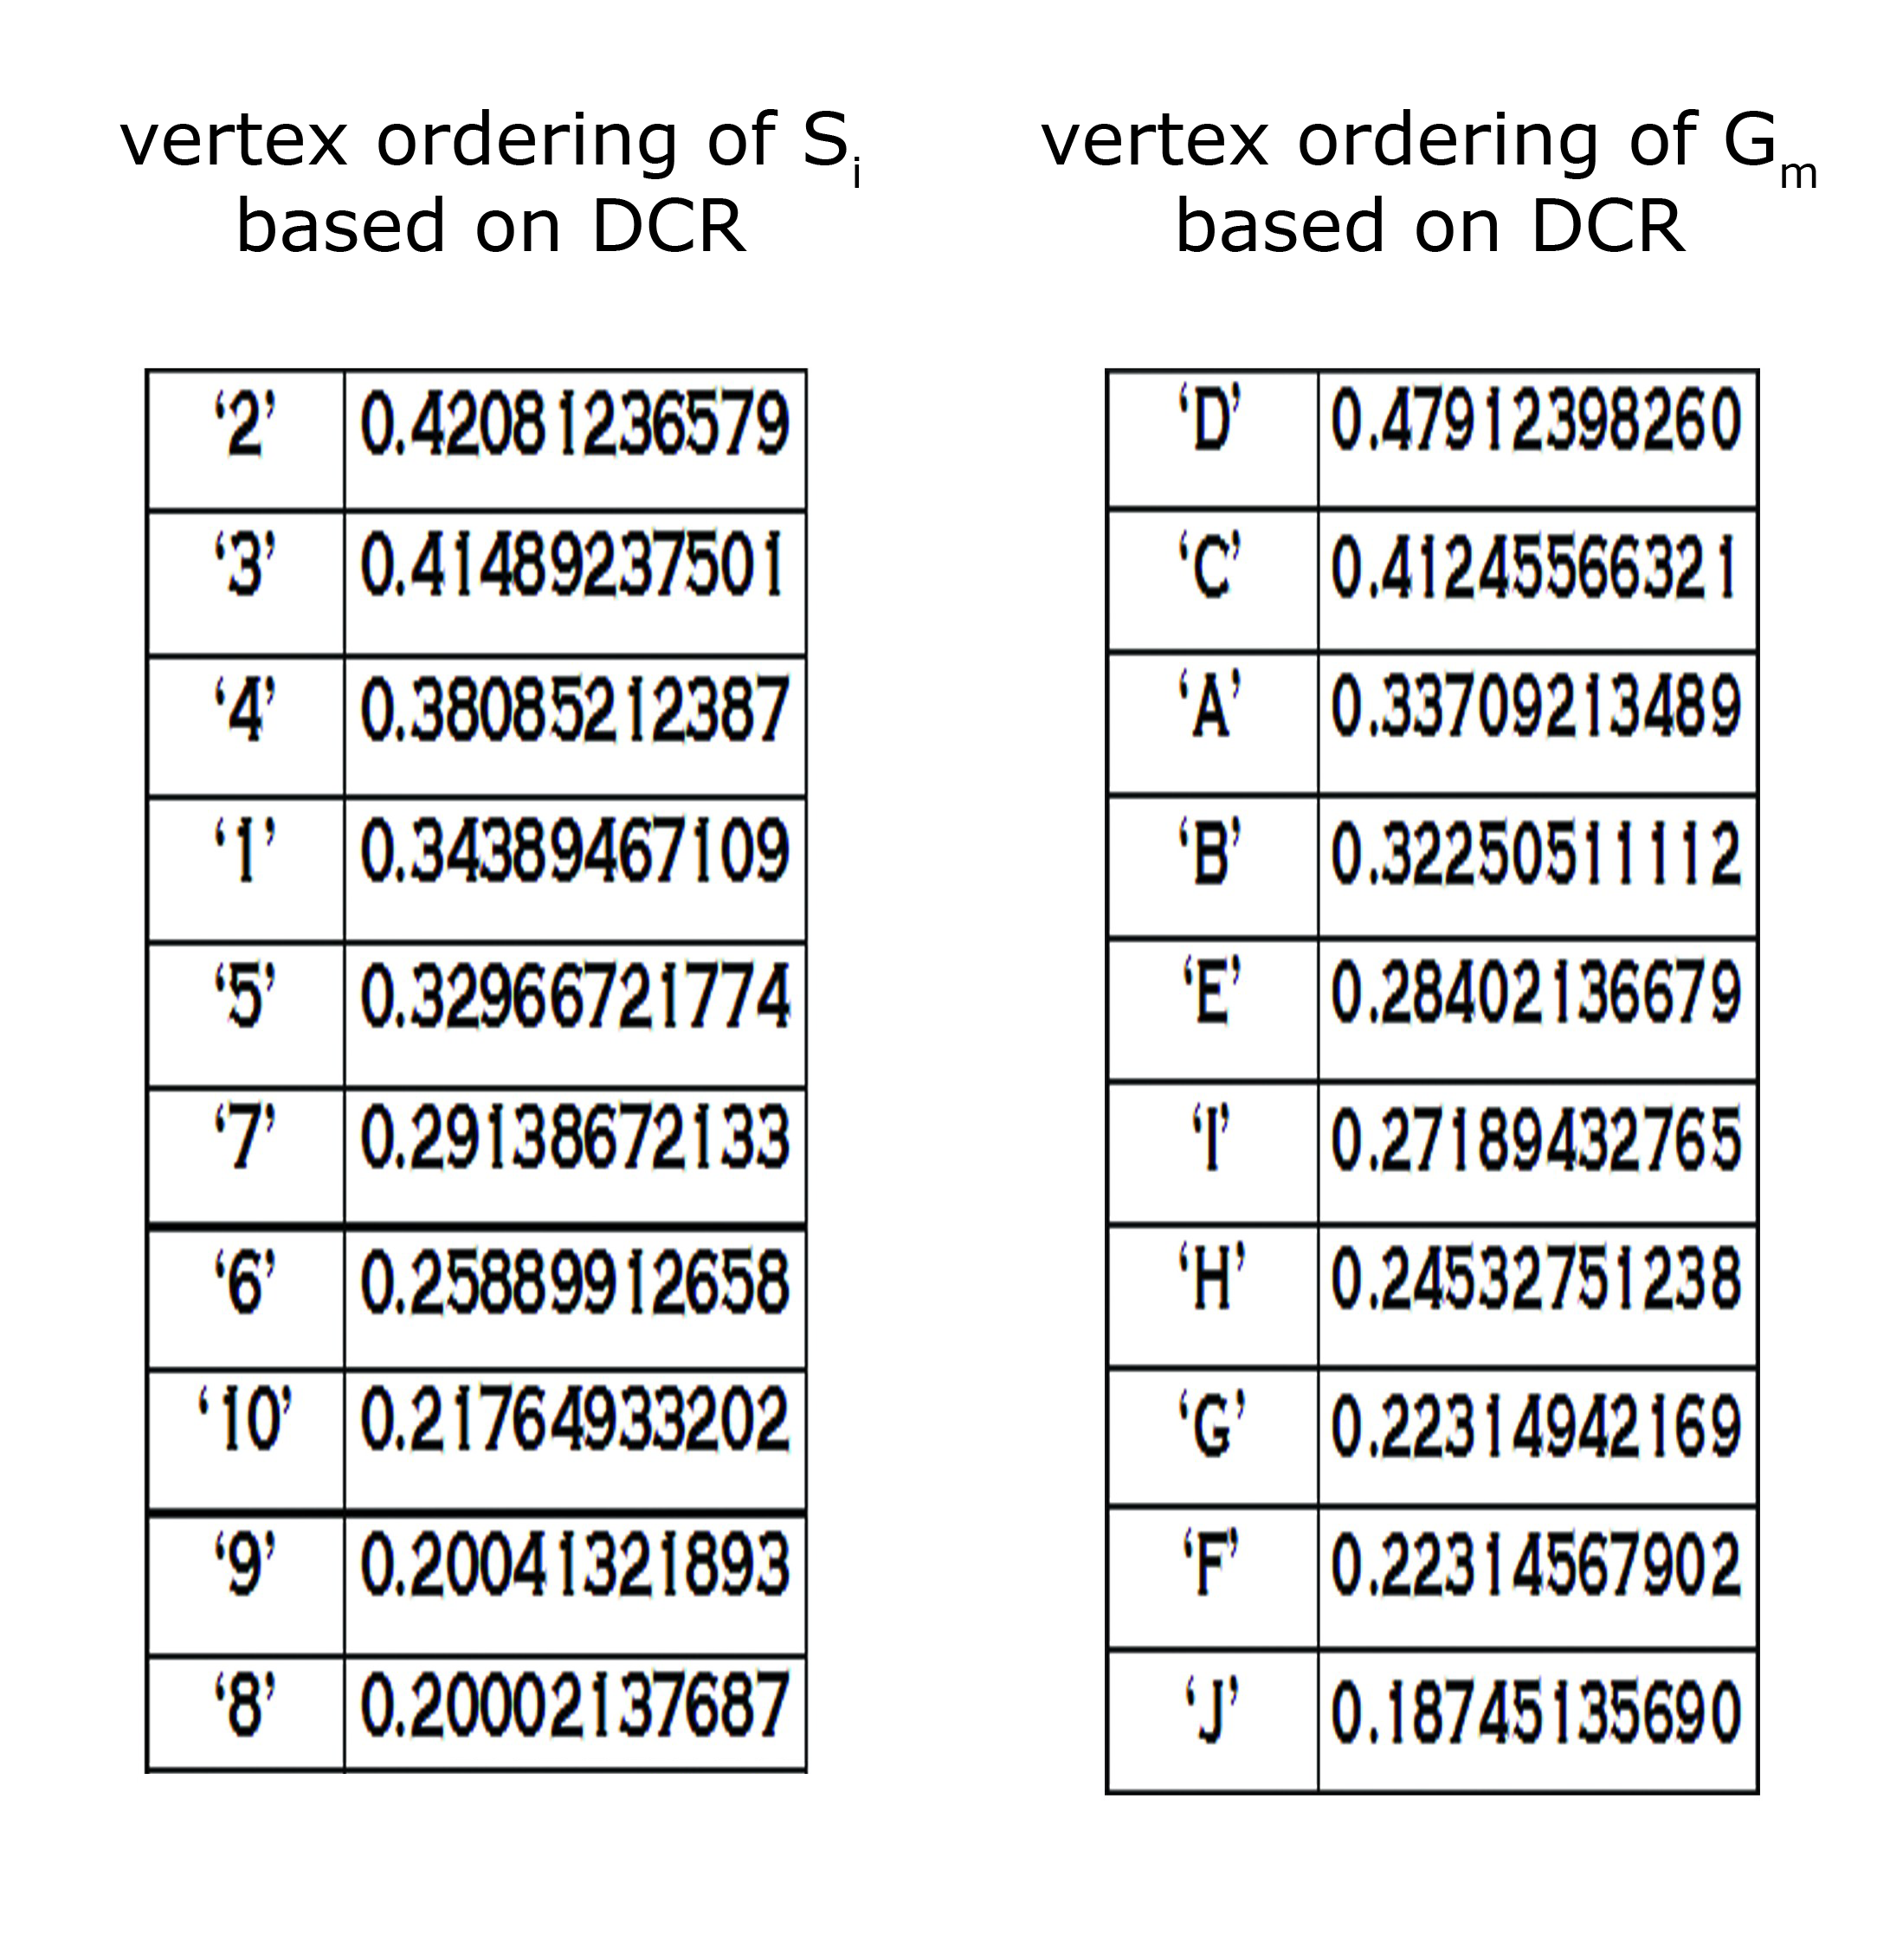
\includegraphics[scale=0.08]{Figures/Mapping_Sorting.jpg}
\caption{}
\label{}
\end{figure}

\begin{figure}[htp]
\centering
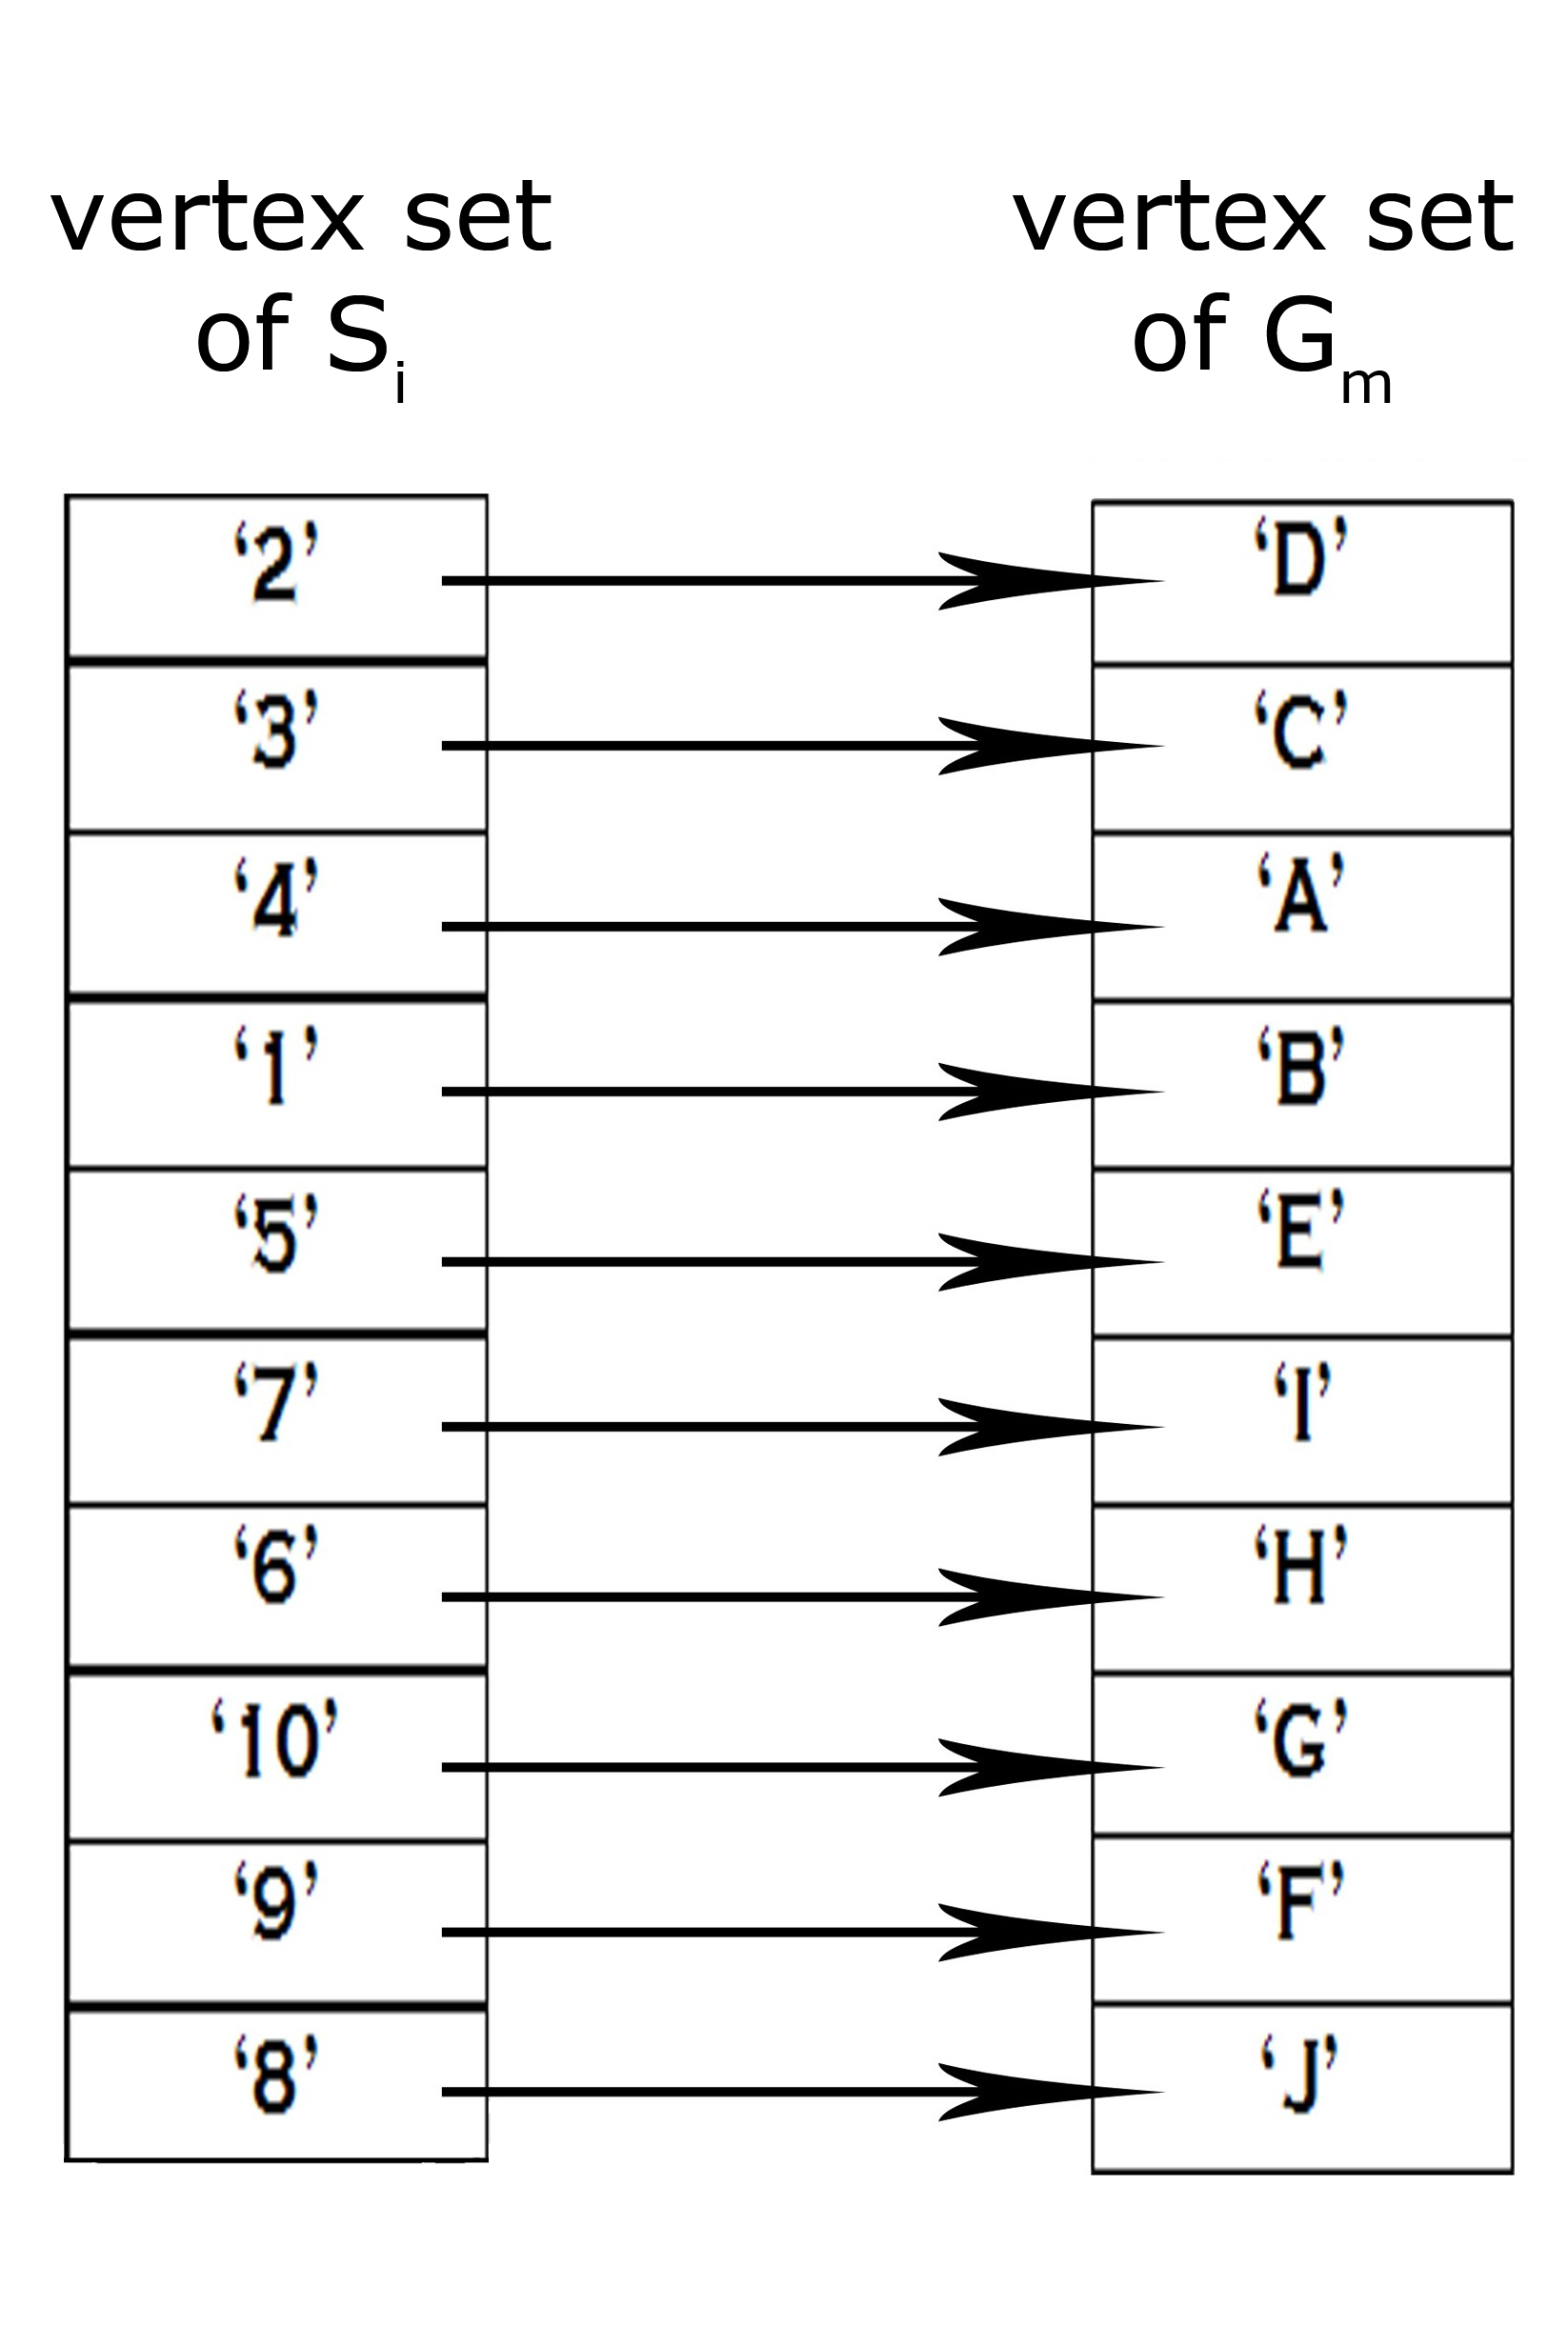
\includegraphics[scale=0.08]{Figures/Mapping_Predicted1.jpg}
\caption{}
\label{}
\end{figure}

\begin{figure}[htp]
\centering
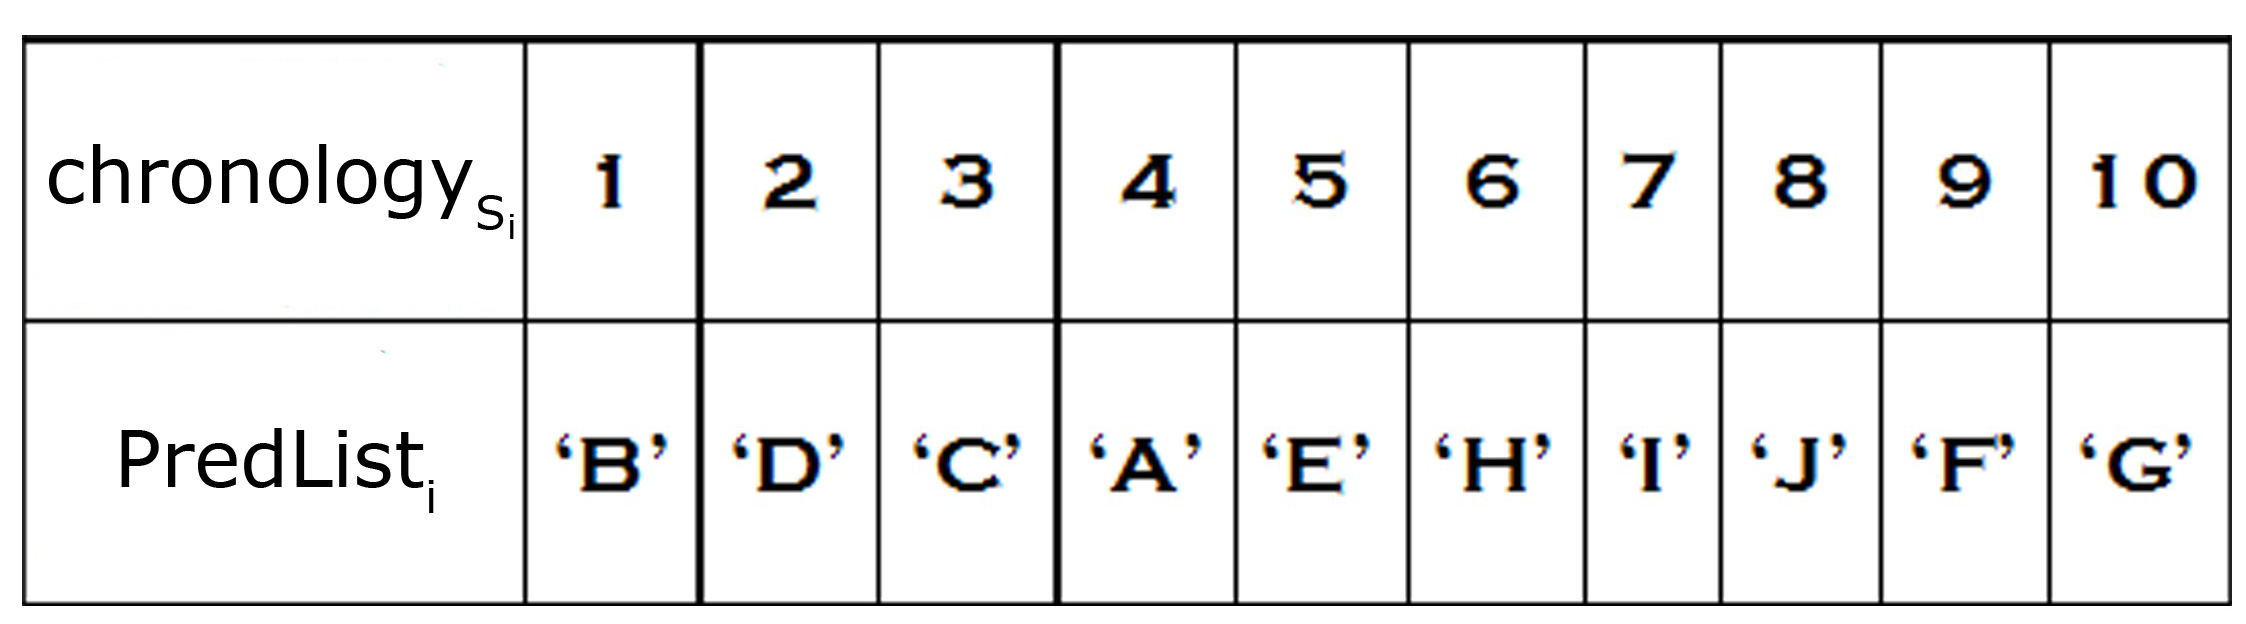
\includegraphics[scale=0.11]{Figures/Mapping_Predicted2.jpg}
\caption{}
\label{}
\end{figure}

This procedure is done for all the sample graphs in the sample space and the final outcome would be $\alpha$ prediction lists.

\subsection{Directed Acyclic Graph}

\hspace{.18in}$\cal D$uring the formation of a network when a new node enters, it attaches itself to one or more existing nodes. Clearly, there is an implicit sense of direction that a new node brings. The main model is no more a undirected graph in this sense, only that the directions are not known in this fully evolved model.
The section aims at arriving at the approximate directed representation of the main model from the $\alpha$ prediction lists derived from the section prior (Mapping).

\subsubsection{S,U,V model }
$\cal T$he model has three parameters.

S : denotes the sample graph.
\\\

u \& v : Any pair of vertices in the main model.
\\\

$\cal T$here are $|V|$ number of nodes. So we have $\alpha \times ^{|V|}C_2$ comparisons or tests to determine the final predicted list. To start with, a pair of nodes $u$ \& $v$ are considered. Note that the original occurrence of the nodes is not known. The ranks of these nodes is noted from each of the $\alpha$ prediction lists. Comparing the ranks of $u$ \& $v$ from $\alpha$ predicted lists we can infer which node arrived prior. Suppose in $\alpha$ comparisons $\kappa$ of them infers $u$ has arrived before $v$ implies $\alpha - \kappa$ of them says $v$ has arrived before $u$.
%Updates so far is that we have as many predicted lists as the number of sample graph. The main aim is to arrive at a final accurate predicted list with the aid of all the predicted lists obtained so far. How can this be done? To start with, a pair of vertices U , V is taken. Note that the original occurrence of the vertices' is not known. The position of the selected vertices in all of these predicted lists is checked. There are two possibilities. Either U has arrived before V or the other way around. We check all the predicted lists and in that we verify, how many times has U arrived before V
\begin{equation}
finalpoints = f = \kappa\ \ \ \ \ \ \ \ \ \ \ \ \  (if\ \kappa > \frac{\alpha}{2})
\end{equation}
\begin{equation}
finalpoints = f = \kappa - \alpha\ \ \ \ \ \ \ \ \ \  (if\ \kappa < \frac{\alpha}{2})
\end{equation}
%Points is assigned the following way.
%\begin{itemize}
%\item If U has arrived before V, points is incremented by 1 unit. 
%\item If V has arrived before U, points is decremented by 1 unit.
%\end{itemize}

Once all the $^{|V|}C_2$ pairs undergoes this process, $finalpoints$ is acquired.
If $finalpoints$ $f$  is positive, U is considered to have come before V. If it is negative, then V is considered to have come before U. But the question is how confident are we about the ordering of every such pair of vertices?  Hence to assure and quantify the confidence level, we introduce a new parameter called the $Confidence Factor$ which is defined as : 
\\\

\bf Hits \rm:  The number of times U arrived before V.
\\\

\bf Misses \rm : The number of times V arrived before U.
\\\

Total No Of Sample Graphs is set by users

\begin{equation}
Confidence factor = CF =\frac{| Total\ number\ of\ Hits- Total\ number\ of\ misses |}{Total\ number\ of\ sample\ graphs} 
\end{equation}

For such $^{|V|}C_2$  pairs of nodes and given $\alpha$ number of graphs say few $\beta$ number of pairs satisfy user specified confidence factor ($CF$) are put in a set say $S$. And for the remaining $^{|V|}C_2 - \beta$ pairs, more sample graphs are created and mapping is done, in-order to verify whether the confidence factor increases or decreases. Those pairs which make up to satisfy $CF$ are put in set $S$. There are possibilities that the confidence level $CF$ is not satisfied even after reaching a generating threshold number of sample graphs.    
%It generates as many number of sample graphs to assert about the ordering of a pair of vertices. Higher the confidence factor, higher the number of sample graphs to cater to the needs of the user’s confident level. There are possibilities that the confidence level is not satisfied even after reaching a $\alpha$ threshold number of sample graphs. So we don’t conclude anything about the pair and move on to check the next pair of vertices. The only reason for this is, there is a lot of entropy in the graph.

\subsection {Drawing Directed Graph}
\subsubsection{Convention}
\hspace{.17in}Now for any pair of vertices from set $S$, the confidence factor $\gamma > CF$. For every pair $(U,V) \in S$, let us assume that V has come after U and it is associated with a confidence factor say $\gamma$. For this pair of vertices a directed edge is drawn from V to U if and only if U has arrived before V.
\begin{figure}[htp]
\centering
\includegraphics[scale=0.30]{Figures/drawing1.png}
\caption{Ideal case : Directed Acyclic Graph ,where there is directed edge for all such $^{|V|}C_2$ pairs of nodes and associated $\gamma = 1$  }
\label{}
\end{figure}

\subsubsection{Effective way of choosing CF :}
For values of $CF \leq .5$ the confidence factor is too low, leads to a scenario that the number of elements in set $S$ will be very high. Which leads to construction of Directed Graph having more number of edges, where accuracy information represented decreases. This results in formation of cycles in the Directed Graph. Clearly demonstrated in the figure 15.
%There is a possibility of the formation of cycles when the $C \leq .5$ which is taken care of by the confidence factor leading to the directed acyclic graph.
\begin{figure}[htp]
\centering
\includegraphics[scale=0.30]{Figures/drawing.png}
\caption{Cycle formation in directed graphs. Nodes 2,6,5,4 and Nodes 4,3,5 form a cycles }
\label{}
\end{figure}

Choosing the confidence factor $CF \geq .80$ leads to a scenario that the number of elements in set $S$ will be less. This leads to construction of Directed Graph which will have less number of edges, therefore the DAG has less information,where the accuracy of information represented is more. This DAG processed further leads to solution where the accuracy will be high and the number of bin($\delta$) formation will be less. Which is not compatible.  

\emph{So Choosing $.5<CF<.8$ gives a optimal solution}

\subsection{The Final Touch}
\subsubsection{The main focus of the method}
\hspace{.17in}$\cal T$he main attribute of the directed graph is the in-degree and the out-degree. We make use of this feature extensively to carry out the further processing. Ideally speaking, the node that has entered first should have no in-degree. On similar note, the node that enters at the end should have no out-degree. Keeping these facts in mind, we move to our Final Step - ‘Binning’
\begin{itemize}
\item Firstly, Here we sort the vertices according to their out degree values and in ascending order for the simple reason that lower the out-degree, earlier it has come. 
\item We have a bunch of vertices with same out-degree. To resolve the ties, we seek the help of yet another characteristic of the DAG which is the in-degree. It is clear that the vertex with higher in-degree has arrived first. Again this not being the ideal case, the bunch of vertices with same out-degree but different in-degree is sorted in descending order and this is done for every such bunch.
\item It so happens that we encounter trouble-making vertices having the same out-degree and in-degree. As it is impossible to fix it, we conclude nothing and simply put such bunch of vertices in one bin. The binned vertices are removed from the existing DAG. Now we have a DAG” graph which will be a induced sub graph of the original DAG. Again we calculate the in-degree and out-degree for the obtained graph and apply same procedure.
\end{itemize} 
Such nodes are removed from the graph and all together we get a new graph which will be a induced sub graph of the Main model. This process is iterated till all the nodes are covered. The order in which the bins are formed is the Final Predicted Order. Finally we have a maximum number of bins and minimal number of elements in each bin.

\section{Conclusion and Further Improvements}
\subsection{Conclusions}
\hspace{.18in} $\cal A$s the number of connections ($C$) in a scale free network
$G=(V,C)$ increases, the accuracy($\eta$) and number of bins($\delta$) increases.   

Proof of correctness is given by the Bin Quality Measure that is exclusively designed to check the accuracy obtained. the plot below gives the necessary details on how our method is better than other methods.

\begin{figure}[htp]
\centering
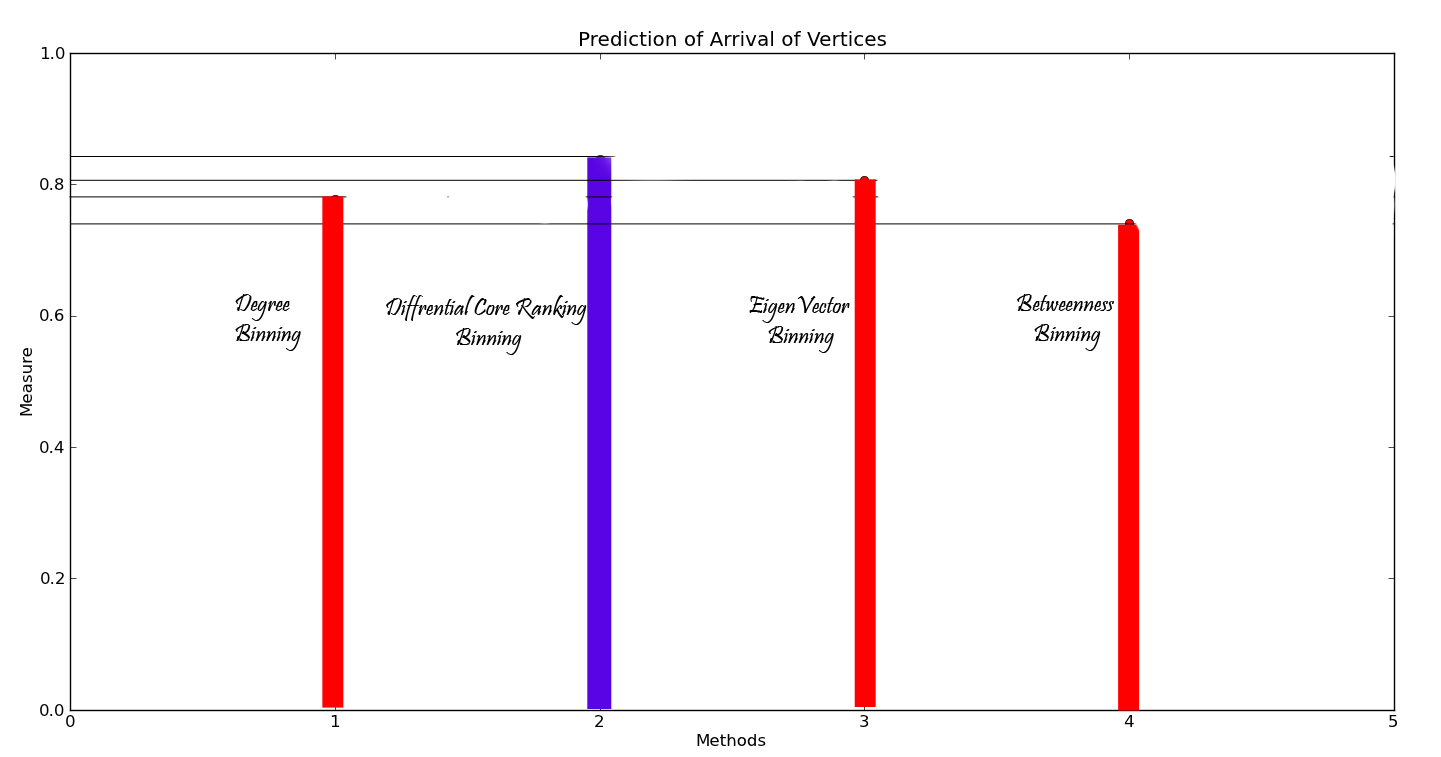
\includegraphics[scale=0.3]{Figures/results1a.jpg}
\caption{Result }
\label{}
\end{figure}

\subsection{Scope and Improvement} 

\hspace{.18in}$\cal S$cale free networks are complex to comprehend in nature and hence prediction of nodes is far from being a trivial task. The best prediction can ofcourse be obtained if a good replication of the main model is generated where the ordering is implicitly known. If the replicated model is found to be close to the main model with respect to properties like degree sequence and other notable characteristics, then there is no necessity of generating the sample space of graphs. By just applying the suv and mapping to the replication, accuracy can be achieved.

But as told earlier due to the complexity and entropy in such networks it becomes hard to replicate the same graph.


\begin{thebibliography}{1}

\bibitem{pois} \url{http://en.wikipedia.org/wiki/Poisson_distribution}

\bibitem{bara1} R.Albert and A.-L.Barab´asi, \emph{Statistical Mechanics of Complex Networks},Rev.Mod.Phys. (2002)[cond-mat/0106096].
\bibitem{bara2} A-L.Barab´asi and R.Albert, Emergence of scaling in random networks, Science (1999).

\end{thebibliography}	
\end{document}

